\section{Iterationen und Meilensteine}
\label{sec:Iterationen und Meilensteine}

\subsection{Iterationsplanung}
Zur Bewältigung dieser Arbeit verwenden wir einen angepassten \acl{RUP} Ablauf. \acs{RUP} definiert 4 Phasen, welche iterativ mehrfach durchlaufen werden.

\begin{itemize}
  \item \textbf{Inception} \newline In der Inception Phase geht es darum, die Details des Arbeitsauftrags auszuarbeiten und ein Fundament für das Projekt zu legen. Dies beinhaltet das Aufsetzen der Projekt-Management Software, erstellen von Repositories \& File-Share. Aber auch das Wählen des Vorgehensmodells.
  \item \textbf{Elaboration 1} \newline In der ersten Elaboration Phase geht es darum sich für eine Programmiersprache und einen Pcap-Wrapper zu entscheiden. Ausserdem wird der Projektplan erstellt und die Dokumentation aufgesetzt.
  \item \textbf{Elaboration 2} \newline In der zweiten Elaboration Phase erstellen wir das Domain Modell sowie einen groben Prototypen unserer Applikation.
  \item \textbf{Construction 1} \newline In der ersten Construction Phase soll die Hälfte der MUSS-Funktionalität implementiert sein. Dies beinhaltet Use Case 1 und Use Case 2.
  \item \textbf{Construction 2} \newline In der zweiten Construction Phase soll die zweite Hälfte der MUSS-Funktionalität implementiert sein. Dies beinhaltet Sub-Use Case 1 und Sub-Use Case 2.
  \item \textbf{Transition} \newline In der Transition-Phase sollen noch allfällige Bugs beseitigt werden, sowie das Usermanual geschrieben und die Präsentation vorbereitet werden. Auch allfällige Rest-Dokumentationsarbeit soll in dieser Phase erledigt werden.
\end{itemize}

\subsection{Meilensteine}
Für das Projekt \tool{} wurden die folgenden Meilensteine festgelegt:

\begin{table}[h]
\centering
\resizebox{\textwidth}{!}{%
\begin{tabular}{|l|l|l|l|}
\hline
\rowcolor[HTML]{C0C0C0} 
\textbf{MS} & \textbf{Name}            & \textbf{Resultat}                                                                                                                                     & \textbf{Datum} \\ \hline
MS1         & Projektplan              & Projektplan erstellt und Iterationen geplant.                                                                                                         & KW12           \\ \hline
MS2         & Anforderungspezifikation & \begin{tabular}[c]{@{}l@{}}Abgeschlossene Anforderungsspezifikationen,\\ Use Cases und ein geplantes Domain Modell für\\ den Prototypen.\end{tabular} & KW13           \\ \hline
MS3         & Erster Prototyp          & \begin{tabular}[c]{@{}l@{}}Ein erster Prototyp als Tech-Demo für das\\ Mitte-Projekt-Meeting mit Open Systems.\end{tabular}                           & KW15           \\ \hline
MS4         & Ende Construction \#1       & Basis Use Cases 1 und 2 implementiert.                                                                                                                & KW17           \\ \hline
MS5         & Ende Construction \#2       & Erweiterte Use Cases 1.1 und 2.1 implementiert.                                                                                                       & KW22           \\ \hline
MS6         & Abgabe SA/BA             & \begin{tabular}[c]{@{}l@{}}Applikation ist fertig für den Release,\\ Dokumentation  wurde abgegeben.\end{tabular}                                                    & KW24           \\ \hline
\end{tabular}
}
\end{table}

\clearpage
\begin{sidewaysfigure}
\centering
\subsection{Zeitplan}
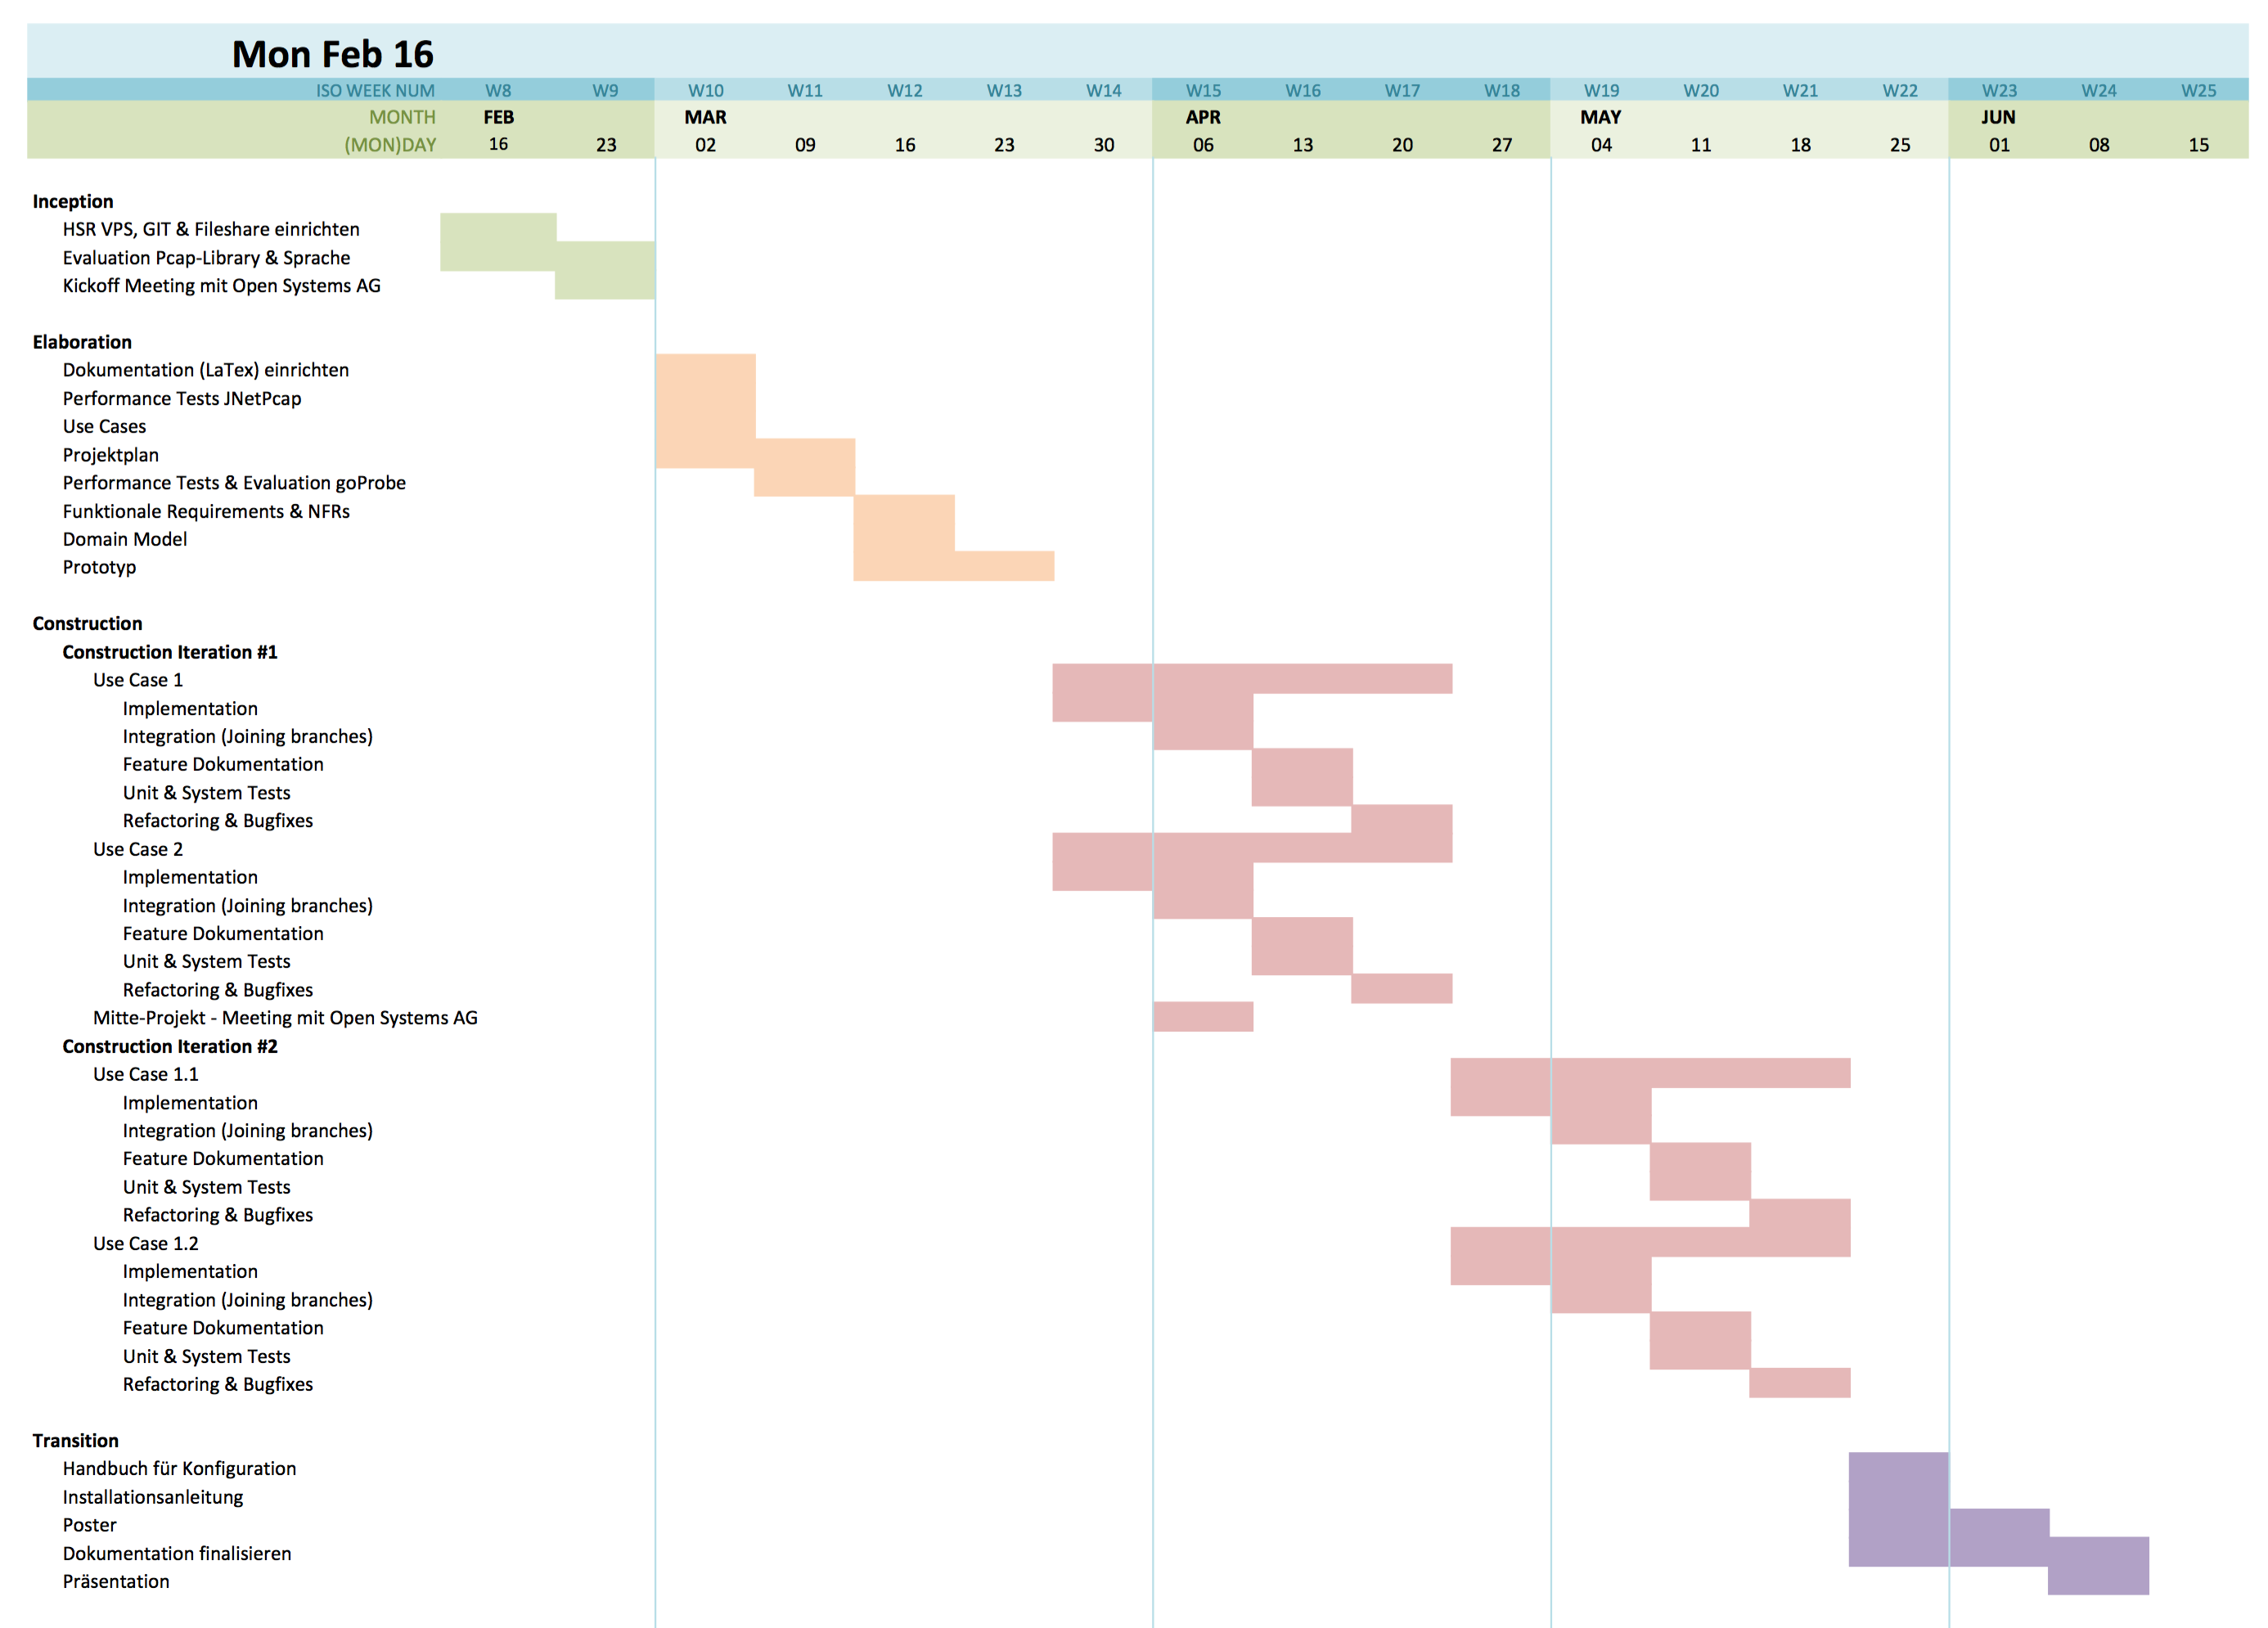
\includegraphics[scale=0.45]{mainpart/projektmanagement/img/ganttdiagramm}
Der Zeitplan wurde in der Elaboration Phase, nach dem Kickoff Meeting, ausgearbeitet und seither nicht mehr verändert. Alle Arbeiten konnten wie geplant durchgeführt werden.
\end{sidewaysfigure}
\clearpage

%\subsection{Arbeitspakete}